\hypertarget{UcRecevoirInfo_8h}{}\section{Référence du fichier src/\+Uc\+Recevoir\+Info.h}
\label{UcRecevoirInfo_8h}\index{src/\+Uc\+Recevoir\+Info.\+h@{src/\+Uc\+Recevoir\+Info.\+h}}
{\ttfamily \#include $<$Serveur\+Tcp\+Com\+Bny.\+h$>$}\newline
{\ttfamily \#include $<$Tcp\+Com\+Bny.\+h$>$}\newline
{\ttfamily \#include $<$iostream$>$}\newline
{\ttfamily \#include $<$stdio.\+h$>$}\newline
{\ttfamily \#include $<$stdlib.\+h$>$}\newline
{\ttfamily \#include $<$string.\+h$>$}\newline
{\ttfamily \#include $<$jsoncpp/json/json.\+h$>$}\newline
{\ttfamily \#include $<$Sqlite\+Persi\+Bny.\+h$>$}\newline
Graphe des dépendances par inclusion de Uc\+Recevoir\+Info.\+h\+:
\nopagebreak
\begin{figure}[H]
\begin{center}
\leavevmode
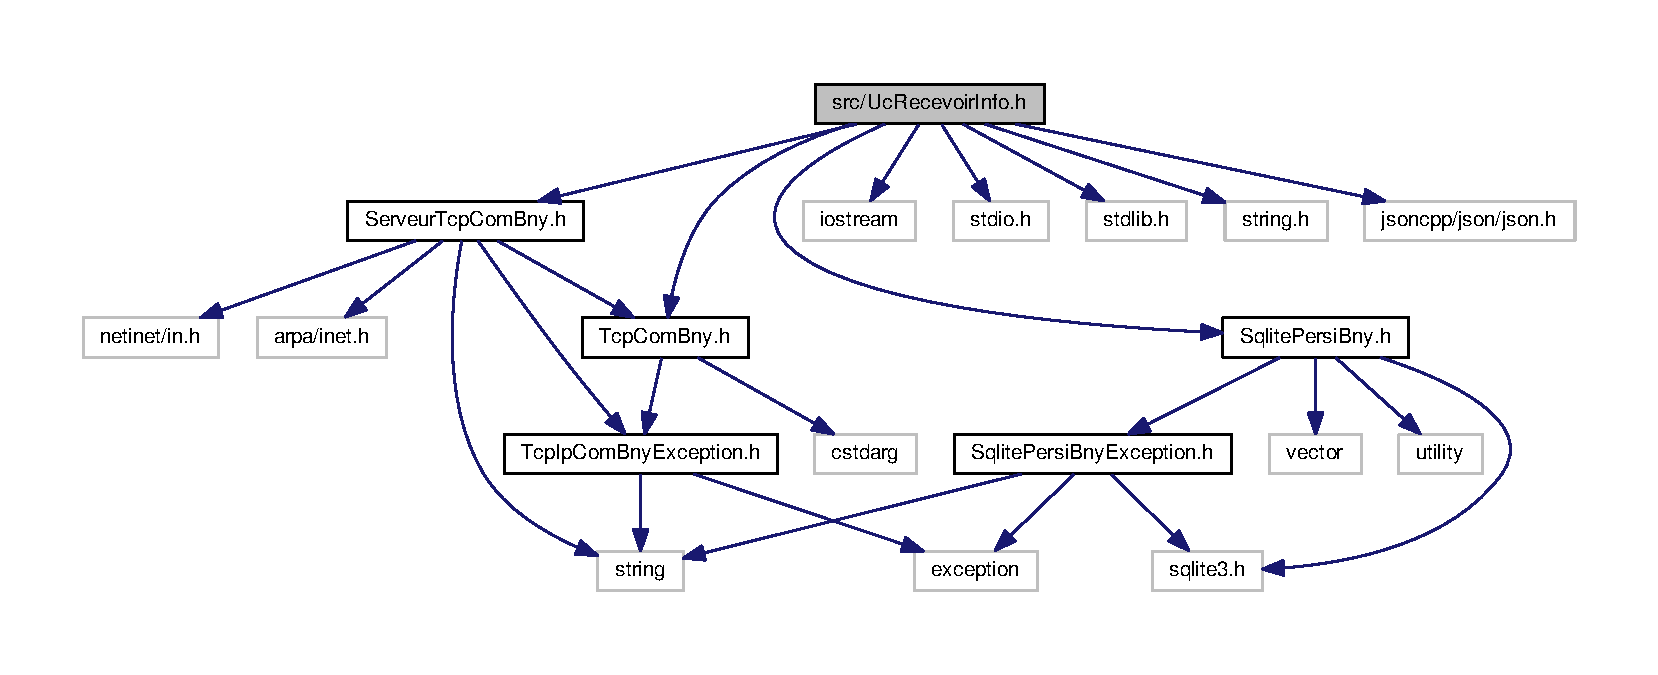
\includegraphics[width=350pt]{UcRecevoirInfo_8h__incl}
\end{center}
\end{figure}
Ce graphe montre quels fichiers incluent directement ou indirectement ce fichier \+:
\nopagebreak
\begin{figure}[H]
\begin{center}
\leavevmode
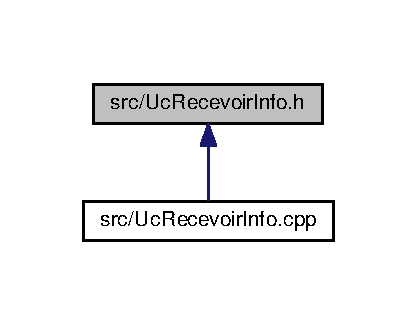
\includegraphics[width=200pt]{UcRecevoirInfo_8h__dep__incl}
\end{center}
\end{figure}
